%% LyX 2.1.4 created this file.  For more info, see http://www.lyx.org/.
%% Do not edit unless you really know what you are doing.
\documentclass[12pt,english]{article}
\usepackage[T1]{fontenc}
\usepackage[latin9]{inputenc}
\usepackage{color}
\usepackage{amsmath}
\usepackage{amsthm}
\usepackage{amssymb}
\usepackage{graphicx}
\usepackage{esint}

\makeatletter
%%%%%%%%%%%%%%%%%%%%%%%%%%%%%% Textclass specific LaTeX commands.
\numberwithin{equation}{section}
\numberwithin{figure}{section}

%%%%%%%%%%%%%%%%%%%%%%%%%%%%%% User specified LaTeX commands.
\usepackage[margin=0.75in]{geometry} % see geometry.pdf on how to lay out the page. There's lots.
\usepackage{graphicx}
\usepackage{cleveref}
\usepackage{amsmath}
\usepackage{multirow}
\usepackage{listings}
\usepackage{color}
\usepackage{CJK}
\definecolor{mygreen}{RGB}{28,172,0}
\definecolor{mylilas}{RGB}{170,55,241}

\usepackage[latin9]{inputenc}
\usepackage{geometry}
\geometry{verbose}


\makeatletter
\@ifundefined{date}{}{\date{}}
\makeatother

%Fancy-header package to modify header/page numbering 
\usepackage{fancyhdr}
\pagestyle{fancy}
\lhead{\textbf{Ge/ESE 118}} %name of the course
\chead{\textbf{}} %topic of the homework set
\rhead{\textbf{Solution 3}} %number of the homework set
\lfoot{}
\cfoot{}
\rfoot{\thepage}


% Matlab script
\lstset{language=Matlab,%
      %basicstyle=\color{red},
  breaklines=true,%
  morekeywords={matlab2tikz},
  keywordstyle=\color{blue},%
  morekeywords=[2]{1}, keywordstyle=[2]{\color{black}},
  identifierstyle=\color{black},%}
  stringstyle=\color{mylilas},
  commentstyle=\color{mygreen},%
  showstringspaces=false,%without this there will be a symbol in the places where there is a space
  numbers=left,%
  numberstyle={\tiny \color{black}},% size of the numbers
  numbersep=9pt, % this defines how far the numbers are from the text
  emph=[1]{for,end,break},emphstyle=[1]\color{red}, %some words to emphasise
                                                      %emph=[2]{word1,word2}, emphstyle=[2]{style},    
}

\makeatother

\usepackage{babel}
\begin{document}

\section*{Problem 1 (graded by Yiran) - 50 points}


\subsection*{(a) 4 points}

In a class, among 20 students, 8 are female, and 12 are male. 2 of
the female students are taller than 170 cm, and 8 of the male students
are taller than 170 cm. Suppose we randomly pick a student, let

$x$: the student is female;

$y$: the student is taller than 170 cm.

Then,

$P(x,y)$ is the probability that the student is both female and is
taller than 170 cm, which is equal to $2/20=0.1$.

$P(x)$ is the probability that the student is female, which is equal
to $8/20=0.4$.

$P(y|x)$ is the probability that known the student is female, she
is taller than 170 cm, which is equal to $2/8=0.25$.

$P(y)$ is the probability that the student is taller than 170 cm,
which is equal to $(2+8)/20=0.5$.

$P(x|y)$ is the probability that known the student is taller than
170 cm, the student is female, which is equal to $2/(2+8)=0.2$.\\
We see that:

$P(x,y)=P(x|y)P(y)=P(y|x)P(x)$


\subsection*{(b) 8 points}

\textbf{\textit{Independent}}\\
Let

$x:$ I get an A for Ge/ESE118.

$y$: The next president of the U.S. is an Republician.

This two events are independent, because $x$ happens, does not affect
the probability of $y$, vice versa.

Let's assume $P(x)=3/5$, and $P(y)=1/2$. 

Suppose I get an A with $P(x)$. It doesn't affect the election at
all, and there is still 1 in 2 odds that the next president will be
an Republician. Therefore, to make both happen, $P(x,y)=P(x)P(y)$.
Similary, suppose the Republician wins the election with $P(y)$.
It doesn't affect my odd to get an A, and to make both happen, $P(x,y)=P(y)P(x)$.

Intuitively, the rule holds because the two events are independent
- one happens does not affect the other; therefore, to make both happen,
we need to multiply $P(x)$ and $P(y)$.\\
\\
\textbf{\textit{Dependent}}\\
Let

$x$: The next president of the U.S. is an Democratic.

$y$: The next president of the U.S. is an Republician.

These two events are not independent, because either of them happens,
will affect the proability of the other. 

Let's assume $P(x)=P(y)=\frac{1}{2}$. Because it's impossible that
the next president is both an Democratic and an Republician, $P(x,y)=0\neq P(x)P(y)$.


\subsection*{(c) 8 points}


\subsection*{(c.i) 3 points}

\begin{eqnarray*}
E(x) & = & \int_{-\infty}^{\infty}xP(x)dx
\end{eqnarray*}


Since $x$ is an odd function, and $P(x)$ is an even function, their
product is an odd function. Integration of an odd function over symmetric
boundaries as $[-\infty,\infty]$ is $0$. Therefore,

\begin{eqnarray*}
E(x)=0
\end{eqnarray*}



\subsection*{(c.ii) 5 points}

\begin{eqnarray*}
E(x^{2}) & = & \int_{-\infty}^{\infty}x^{2}P(x)dx\\
 & = & \int_{-\infty}^{\infty}x^{2}\frac{1}{\sigma\sqrt{2\pi}}\exp\left(-\frac{x^{2}}{2\sigma^{2}}\right)dx
\end{eqnarray*}


Since

\begin{eqnarray*}
\left[\exp\left(-\frac{x^{2}}{2\sigma^{2}}\right)\right]' & = & -\frac{x}{\sigma^{2}}\exp\left(-\frac{x^{2}}{2\sigma^{2}}\right)
\end{eqnarray*}


Then

\begin{eqnarray*}
E(x^{2}) & = & -\frac{\sigma}{\sqrt{2\pi}}\int_{-\infty}^{\infty}x\left[\exp\left(-\frac{x^{2}}{2\sigma^{2}}\right)\right]'dx\\
 & = & -\frac{\sigma}{\sqrt{2\pi}}\left[x\exp\left(-\frac{x^{2}}{2\sigma^{2}}\right)\bigg|_{-\infty}^{\infty}-\int_{-\infty}^{\infty}\exp\left(-\frac{x^{2}}{2\sigma^{2}}\right)dx\right]\\
 & = & \frac{\sigma}{\sqrt{2\pi}}\int_{-\infty}^{\infty}\exp\left(-\frac{x^{2}}{2\sigma^{2}}\right)dx\\
\end{eqnarray*}


Since

\begin{eqnarray*}
\int_{-\infty}^{\infty}e^{-x^{2}/2}dx & = & \sqrt{2\pi}\\
 & = & \int_{-\infty}^{\infty}\exp\left[-\frac{\left(\frac{x}{\sigma}\right)^{2}}{2}\right]d\left(\frac{x}{\sigma}\right)\\
 & = & \frac{1}{\sigma}\int_{-\infty}^{\infty}\exp\left(-\frac{x^{2}}{2\sigma^{2}}\right)dx
\end{eqnarray*}


Then

\begin{eqnarray*}
E(x^{2}) & = & \frac{\sigma}{\sqrt{2\pi}}\sqrt{2\pi}\sigma=\sigma^{2}
\end{eqnarray*}



\subsection*{(d) 30 points}


\subsection*{(d.i) 10 points}

\begin{eqnarray*}
P(d_{i}|L) & = & \frac{3}{4}\mathcal{\mathcal{N}}(L,\sigma)+\frac{1}{4}\mathcal{N}(L+1,\sigma)\\
 & = & \frac{3}{4}\frac{1}{\sigma\sqrt{2\pi}}\exp\left(-\frac{(d_{i}-L)^{2}}{2\sigma^{2}}\right)+\frac{1}{4}\frac{1}{\sigma\sqrt{2\pi}}\exp\left(-\frac{(d_{i}-(L+1))^{2}}{2\sigma^{2}}\right)\\
 & = & \frac{15}{2}\frac{1}{\sqrt{2\pi}}\exp\left(-50(d_{i}-L)^{2}\right)+\frac{3}{2}\frac{1}{\sqrt{2\pi}}\exp\left(-50(d_{i}-(L+1))^{2}\right)
\end{eqnarray*}


where $\sigma=0.1$ cm, and $L$, $d_{i}$ are in cm.

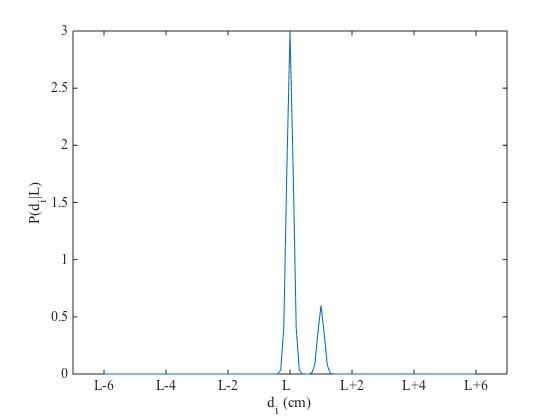
\includegraphics[scale=0.8]{p1_figures/d_i}


\subsection*{(d.ii) 10 points}

From Bayes' theorem,

\begin{eqnarray*}
P(L|d_{i}) & = & \frac{P(d_{i}|L)P(L)}{P(d_{i})}\\
 & \propto & P(d_{i}|L)=\frac{3}{4}\frac{1}{\sigma\sqrt{2\pi}}\exp\left(-\frac{(d_{i}-L)^{2}}{2\sigma^{2}}\right)+\frac{1}{4}\frac{1}{\sigma\sqrt{2\pi}}\exp\left(-\frac{(d_{i}-(L+1))^{2}}{2\sigma^{2}}\right)
\end{eqnarray*}


Where we assume the prior distribution $P(L)$ is uniform, and $P(d_{i})$
is a constant (but different for different $d_{i}$). 

The constant ahead of $P(d_{i}|L)$ (denoted as ``$c$'') is determined
by

\begin{eqnarray*}
\int_{-\infty}^{\infty}P(L|d_{i})dL & =\text{\ensuremath{\int}}_{-\infty}^{\infty}cP(d_{i}|L)dL & =1\\
\end{eqnarray*}


We can re-write $P(d_{i}|L)$ as

\begin{eqnarray*}
P(d_{i}|L) & = & \frac{3}{4}\frac{1}{\sigma\sqrt{2\pi}}\exp\left(-\frac{(L-d_{i})^{2}}{2\sigma^{2}}\right)+\frac{1}{4}\frac{1}{\sigma\sqrt{2\pi}}\exp\left(-\frac{(L-(d_{i}-1))^{2}}{2\sigma^{2}}\right)
\end{eqnarray*}


which is a summation of two normal distributions (centered at $d_{i}$,
and $d_{i}-1$), weighted by $\frac{3}{4}$ and $\frac{1}{4}$.

Then

\begin{eqnarray*}
\int_{-\infty}^{\infty} & P(d_{i}|L)dL & =1
\end{eqnarray*}


Therefore, the constant $c=1$ 

\begin{eqnarray*}
P(L|d_{i}) & = & P(d_{i}|L)\\
 & = & \frac{3}{4}\frac{1}{\sigma\sqrt{2\pi}}\exp\left(-\frac{(L-d_{i})^{2}}{2\sigma^{2}}\right)+\frac{1}{4}\frac{1}{\sigma\sqrt{2\pi}}\exp\left(-\frac{(L-(d_{i}-1))^{2}}{2\sigma^{2}}\right)\\
 & = & \frac{15}{2}\frac{1}{\sqrt{2\pi}}\exp\left(-50(L-d_{i})^{2}\right)+\frac{3}{2}\frac{1}{\sqrt{2\pi}}\exp\left(-50(L-(d_{i}-1))^{2}\right)
\end{eqnarray*}


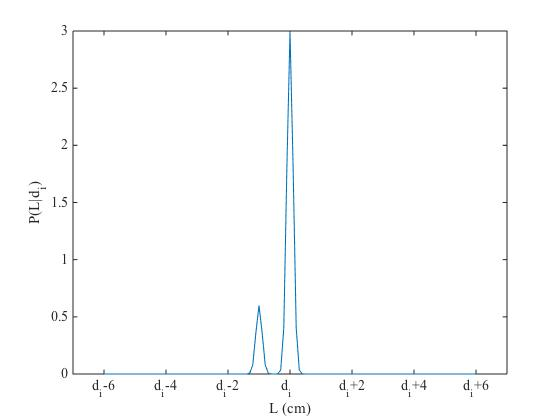
\includegraphics[scale=0.8]{p1_figures/d_ii}


\subsection*{(d.iii) 10 points}

We can use the distribution of $L$ from the first measurement as
prior distribution to compute a posterior distribution after the second
measurement
\begin{eqnarray*}
P(L|d_{1}=8.3,d_{2}=9.1) & \propto & P(d_{2}=9.1|L)P(L|d_{1}=8.3)\\
\end{eqnarray*}


Since we only care about the maximum of the LHS, instead of its value;
for the RHS, absortbing the $\frac{1}{4}\frac{1}{\sigma\sqrt{2\pi}}$
terms into the constant

\begin{eqnarray*}
P(L|d_{1}=8.3,d_{2}=9.1) & \propto & \left[3\exp\left(-50(9.1-L)^{2}\right)+\exp\left(-50(8.1-L)^{2}\right)\right]\\
 &  & \cdot\left[3\exp\left(-50(L-8.3)^{2}\right)+\exp\left(-50(L-7.3))^{2}\right)\right]
\end{eqnarray*}


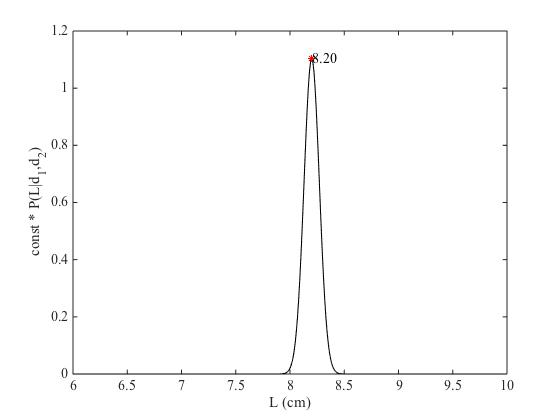
\includegraphics[scale=0.8]{p1_figures/d_iii}

From the plot, we see that the best estimate of $L$ is $8.2$. 

Because the two measurement differs $\approx1$, it's likely that
in the second measurement, the one quarter chance of additional 1
cm happens. After the 1 cm correction, the second measurement should
be 8.1. The mean of 8.3 and 8.1 is 8.2, which is our estimation through
the analysis above.

\newpage{}


\section*{Problem 2 (graded by Kangchen) - 50 points}


\subsection*{(a)12 points}

$P(\boldsymbol{m})\propto e^{-F(\boldsymbol{m})}$where $F(\boldsymbol{m})=\sum\frac{(d_{k}-g_{k}(\boldsymbol{m}))^{2}}{2\sigma_{k}^{2}}$ 


\subsection*{(b)12 points}

Since $d'_{k}=d_{k}/\sigma_{k}$, the relation between $\boldsymbol{d}'$
and $\boldsymbol{d}$ can be written in matrix form $\boldsymbol{d}'=\boldsymbol{W}\boldsymbol{d}$
where $W_{ij}=\delta_{ij}\frac{1}{\sigma_{j}}$ ($\delta_{ij}=1$
if $i=j$ , $\delta_{ij}=0$ if $i\neq j$).


\subsection*{(c)12 points\textcolor{black}{
\[
F=\frac{1}{2}(\boldsymbol{d'-g'}(\boldsymbol{m}))^{T}(\boldsymbol{d'-g}'(\boldsymbol{m}))
\]
}}

the gradient: $\boldsymbol{\nabla}F=\hat{\boldsymbol{G}'}^{T}(\boldsymbol{d}'-\boldsymbol{g}'(\boldsymbol{m}))$

the approximated hessian: $\boldsymbol{H}=(\hat{\boldsymbol{G}'}^{T}\hat{\boldsymbol{G}'})$

So the least squares solution: $\Delta\boldsymbol{m}=(\hat{\boldsymbol{G}'}^{T}\hat{\boldsymbol{G}'})^{-1}\hat{\boldsymbol{G}'}^{T}(\boldsymbol{d}'-\boldsymbol{g}'(\boldsymbol{m}))$

Substitute $\hat{\boldsymbol{G}'}=\boldsymbol{W}\hat{\boldsymbol{G}}$,
$\boldsymbol{d}'=\boldsymbol{W}\boldsymbol{d}$, $\boldsymbol{g}'=\boldsymbol{W}\boldsymbol{g}$,
$\boldsymbol{C}=\boldsymbol{W}^{T}\boldsymbol{W}$

$\Delta\boldsymbol{m}=(\hat{\boldsymbol{G}}^{T}\boldsymbol{W}^{T}\boldsymbol{W}\hat{\boldsymbol{G}})^{-1}\hat{\boldsymbol{G}}^{T}\boldsymbol{W}^{T}\boldsymbol{W}(\boldsymbol{d}-\boldsymbol{g}(\boldsymbol{m}))=(\hat{\boldsymbol{G}}^{T}\boldsymbol{C}\hat{\boldsymbol{G}})^{-1}\hat{\boldsymbol{G}}^{T}\boldsymbol{C}(\boldsymbol{d}-\boldsymbol{g}(\boldsymbol{m}))$


\subsection*{(d)14 points\tiny
\lstinputlisting{./HW3_Q1/compute_gradient_approx_hess.m}
\normalsize\tiny
\lstinputlisting{./HW3_Q1/nonlinear_solver.m}
\normalsize\tiny
\lstinputlisting{./HW3_Q1/compute_residue.m}
\normalsize\tiny
\lstinputlisting{./HW3_Q1/HW3_Q1.m}
\normalsize}

\[
\boldsymbol{m}=[8.3068,-5.3425,11.8179,31.8569]^{T}
\]


\[
\boldsymbol{error}=[-4.99\times10^{-5},1.20\times10^{-5}-2.95\times10^{-3},3.59\times10^{-4},-2.87\times10^{-5},2.74\times10^{-6}]
\]


We can find that since we put a smaller weight on station 3, its error
is the largest.

Since we put a larger weight on station 5 6 , their errors are smaller.

\newpage{}


\section*{(Extra Credit) Problem 3 (graded by Yiran) - 25 points}


\subsection*{(a) 5 points}

Since $\boldsymbol{g_{i}}$ has M elements, the maximum dimension
of $\boldsymbol{G}$ spanned by $\{\boldsymbol{g_{i}},i=1...N\}$
is M. Therefore,

\begin{eqnarray*}
dim\left(R(\boldsymbol{G})\right) & \leq & M<N=dim(\mathbb{R}^{N})
\end{eqnarray*}



\subsection*{(b) 10 points}

\begin{eqnarray*}
\boldsymbol{H_{ij}} & = & \boldsymbol{g_{i}}^{T}\boldsymbol{g_{j}}
\end{eqnarray*}


The diagonal elements of $\boldsymbol{H}$ are the squared lengths
of the column vectors of $\boldsymbol{G}$, the off-diagnoal elements
measure how much the column vectors of $\boldsymbol{G}$ project onto
each other. Suppose we project a vector $\boldsymbol{d}$ into the
column space of $\boldsymbol{G}$, the coordinates are $(m_{1},...,m_{M})$.
If the length of certain column vector $\boldsymbol{g_{i}}$ is small,
an error in $\boldsymbol{d}$ will cause a big error in $m_{i}$.
The error in $\boldsymbol{d}$ also tends to affect those $m_{i}$
similarly if their corresponding column vectors $\boldsymbol{g_{i}}$
are near parallel.


\subsection*{(c) 5 points}

\begin{eqnarray*}
\boldsymbol{G}^{T}\boldsymbol{d} & = & (\boldsymbol{g_{1}}^{T}\boldsymbol{d},...,\boldsymbol{g_{M}}^{T}\boldsymbol{d})^{T}
\end{eqnarray*}


which is the projection of $\boldsymbol{d}$ into the model space.


\subsection*{(d) 5 points}

This equation implies that $\boldsymbol{Gm}$ equals the projection
of $\boldsymbol{d}$ in the model space. Thus, the least-squares solution
$\boldsymbol{m}$ is the coordinate of $\boldsymbol{d}$ in the model
space.
\end{document}
